\documentclass[conference]{IEEEtran}
\IEEEoverridecommandlockouts
% The preceding line is only needed to identify funding in the first footnote. If that is unneeded, please comment it out.
\usepackage{cite}
\usepackage{amsmath,amssymb,amsfonts}
\usepackage{algorithmic}
\usepackage{graphicx}
\usepackage{textcomp}
\usepackage{xcolor}
\def\BibTeX{{\rm B\kern-.05em{\sc i\kern-.025em b}\kern-.08em
    T\kern-.1667em\lower.7ex\hbox{E}\kern-.125emX}}
\begin{document}

\title{Simple CNN from scratch}



\author{\IEEEauthorblockN{Phi Doan Minh Luong}
\IEEEauthorblockA{2440046}
}

\maketitle

\begin{abstract}
This project uses the MNIST dataset to present a from-scratch implementation of a basic CNN architecture.  The network, which consists of a dense layer with a softmax output, a max-pooling layer, a convolutional layer, and a ReLU activation function, is built completely in Python without the use of machine learning or numerical computation libraries.
\end{abstract}

\begin{IEEEkeywords}
CNN, MNIST, Deep learning
\end{IEEEkeywords}

\section{Introduction}
Convolution Neural Networks (CNNs) have revolutionized the field of computer vision, achieving state-of-the-art performance in tasks such as image classification, object detection, and image segmentation. Their architecture, inspired by the human visual cortex, effectively captures hierarchical patterns in visual data through a series of specialized layers, including convolutional, pooling, and fully connected layers. The widespread availability of powerful deep learning frameworks like TensorFlow, PyTorch, and Keras has made the development and deployment of complex CNN models more accessible than ever.

However, the abstraction provided by these libraries, while beneficial for rapid prototyping, can often obscure the fundamental mechanisms that drive these networks. A deep understanding of the underlying mathematical operations, data flow, and gradient computations during backpropagation is invaluable for researchers and practitioners aiming to innovate, debug, or optimize neural network models. Motivated by this, the work presented in this project focuses on implementing a simple CNN from its foundational components without the aid of such high-level libraries.

This project's main goal is to create, put into practice, and evaluate a simple CNN architecture that can recognize handwritten numbers from the popular MNIST dataset. We try to expose the pre-built neural network components by building each layer—convolution, ReLU activation, max pooling, and dense (totally connected)—as well as the backpropagation algorithm using only common Python data structures and control flow.

The key contributions of this project are:
\begin{itemize}
    \item A detailed, step-by-step implementation of core CNN layers and their associated forward and backward pass computations in pure Python.
    \item A functional demonstration of the implemented CNN's ability to train on the MNIST dataset and perform digit classification.
    \item An analysis of the computational performance and challenges inherent in a from-scratch implementation, providing context for the efficiency of optimized numerical libraries.
    \item Educational insights into the intricate workings of CNNs, particularly the gradient flow during backpropagation, which are often abstracted away by modern frameworks.
\end{itemize}


\section{Background}
\subsection{Convolutional Neural Networks (CNNs)}
CNNs are a class of deep neural networks particularly well-suited for processing grid-like data, such as images. Their architecture typically consists of several key types of layers:

\begin{itemize}
    \item \textbf{Convolutional Layer:} This is the core building block of a CNN. It applies a set of learnable filters (kernels) to the input image (or feature map from a previous layer). Each filter slides across the input, computing the dot product between the filter entries and the input at each position. This operation produces a 2D activation map, or feature map, highlighting specific features (e.g., edges, textures) detected by the filter. Key parameters include the number of filters, kernel size, stride (step size of the filter), and padding (adding zeros around the input border).

    \item \textbf{Activation Function:} Applied element-wise after the convolution operation (and often after dense layers), activation functions introduce non-linearity into the network, enabling it to learn more complex patterns. Common choices include the Rectified Linear Unit (ReLU), defined as $f(x) = \max(0, x)$, which is computationally efficient and helps mitigate the vanishing gradient problem. Other functions like Sigmoid or Tanh are also used.

    \item \textbf{Pooling Layer (Subsampling):} Pooling layers reduce the spatial dimensions (width and height) of the feature maps, thereby reducing the number of parameters and computation in the network. This also helps to make the representation more robust to small translations in the input. Max Pooling is a common type, where a filter slides over the input feature map and outputs the maximum value within each receptive field.

    \item \textbf{Flatten Layer:} After several convolutional and pooling layers, the high-level feature maps are typically flattened into a one-dimensional vector. This vector then serves as the input to one or more fully connected layers.

    \item \textbf{Fully Connected (Dense) Layer:} In a dense layer, every neuron is connected to every neuron in the previous layer. These layers perform classification based on the features extracted by the preceding convolutional and pooling layers.

    \item \textbf{Softmax Layer:} For multi-class classification tasks, the output layer typically uses a softmax activation function. Softmax converts a vector of raw scores (logits) into a probability distribution over the K output classes, where each element represents the probability that the input belongs to a particular class.
\end{itemize}

\subsection{MNIST Dataset}
The MNIST (Modified National Institute of Standards and Technology) dataset is a widely used benchmark for image classification tasks. It consists of 70,000 grayscale images of handwritten digits (0 through 9), each of size 28x28 pixels. The dataset is pre-divided into a training set of 60,000 images and a test set of 10,000 images. Its simplicity and well-defined structure make it an ideal choice for developing and testing new machine learning algorithms, particularly for educational purposes and for implementing models from scratch.

\subsection{From-Scratch Implementation Rationale}
Modern deep learning libraries like TensorFlow and PyTorch provide highly optimized, pre-built components for constructing neural networks. While these tools accelerate development, they abstract away many of the underlying details. Implementing a CNN "from scratch," using only fundamental programming constructs and without relying on these specialized libraries (or even numerical computation libraries like NumPy for core tensor operations), offers several benefits:
\begin{itemize}
    \item \textbf{Deeper Understanding:} It forces a detailed engagement with the mathematical operations within each layer, the data flow, and the intricacies of the backpropagation algorithm.
    \item \textbf{Demystification:} It helps to demystify what happens "under the hood" of high-level library functions.
    \item \textbf{Appreciation of Complexity:} It provides an appreciation for the computational challenges and optimizations handled by dedicated libraries.
\end{itemize}
The purposeful application of this from-scratch method in this project understands the inherent trade-off in computing efficiency as compared to library-based methods and focuses on these core learning elements.

\section{Proposed CNN Architecture and Implementation}
\subsection{Overall Network Architecture}
The proposed CNN architecture is intentionally kept simple to focus on the fundamental building blocks. It consists of a single convolutional layer followed by a ReLU activation, a max-pooling layer, a flatten operation, and a fully connected (dense) output layer with a softmax activation. All the configurations of the CNN can be changed by using the "config.txt" file. The data flow through the network is as follows:

\begin{enumerate}
    \item \textbf{Input}: Grayscale MNIST images of size 28x28 pixels.
    \item \textbf{Convolutional Layer (C1)}:
        \begin{itemize}
            \item Input: 1 channel (grayscale), 28x28 image.
            \item Filters: 3 filters.
            \item Kernel Size: 5x5.
            \item Stride: 1.
            \item Padding: 'Valid' (no padding applied by the layer itself).
            \item Output: 3 feature maps, each of size (28-5)/1 + 1 = 24x24.
        \end{itemize}
    \item \textbf{ReLU Activation (A1)}: Applied element-wise to the output of the convolutional layer C1.
    \item \textbf{Max Pooling Layer (P1)}:
        \begin{itemize}
            \item Input: 3 feature maps, each 24x24.
            \item Pool Size: 2x2.
            \item Stride: 2.
            \item Output: 3 feature maps, each of size 24/2 = 12x12.
        \end{itemize}
    \item \textbf{Flatten Layer}: The 3 feature maps of size 12x12 are flattened into a single vector of size 3 * 12 * 12 = 432.
    \item \textbf{Dense Output Layer (F1)}:
        \begin{itemize}
            \item Input: Vector of size 432.
            \item Neurons: 10 (one for each MNIST digit class 0-9).
            \item Activation: Linear output (logits).
        \end{itemize}
    \item \textbf{Softmax Activation}: Applied to the output of the dense layer F1 to produce a probability distribution over the 10 classes.
\end{enumerate}

A conceptual diagram of this architecture is shown in this figure

\begin{figure}[htbp]
    \centering
    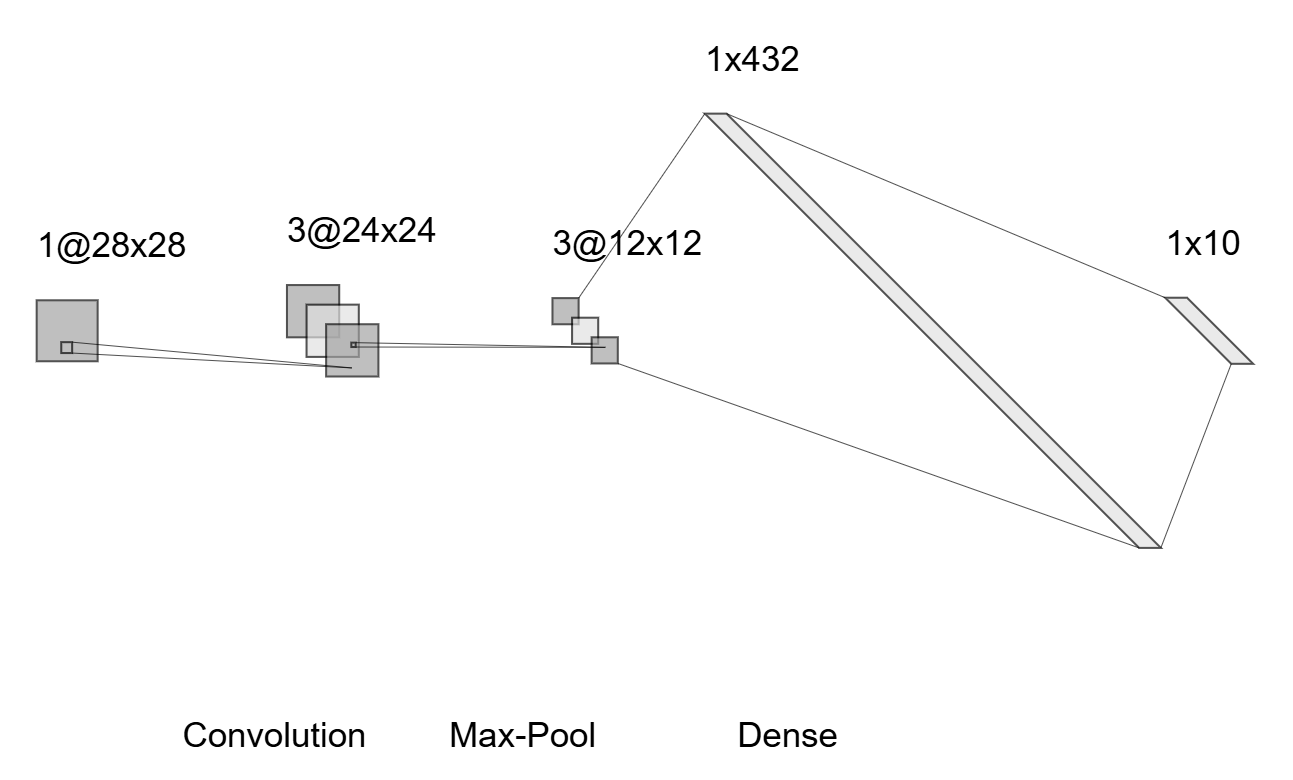
\includegraphics[width=0.9\columnwidth]{architecture.png}
    \caption{Conceptual diagram of the proposed simple CNN architecture.}
    \label{fig:cnn_architecture}
\end{figure}

\subsection{Layer Implementation Details}
All layers are implemented using standard Python lists to represent tensors (multi-dimensional arrays) and basic arithmetic operations.

\subsubsection{Convolutional Layer (Conv2D)}
\begin{itemize}
    \item \textbf{Forward Pass}: For each output feature map, its corresponding 5x5 kernel slides across all input channels of the 28x28 input image with a stride of 1. At each position, an element-wise multiplication between the kernel and the overlapping input region is performed, and the results are summed. This result is the pre-activation value for one element in the output feature map. To simplify, we don't use bias for the convolutional layer.
    \item \textbf{Backward Pass}: Gradients are computed for the layer's weights (kernels), and its input.
        \begin{itemize}
            \item $\partial L / \partial W_{k}$: The gradient of the loss $L$ with respect to a kernel weight $W_{k}$ is calculated by summing the product of the incoming gradient from the subsequent layer (post-activation) and the corresponding input activation values that contributed to that output during the forward pass.
            \item $\partial L / \partial X_{in}$: The gradient with respect to the layer's input $X_{in}$ (to be passed to the previous layer) is computed by a full convolution operation between the incoming gradient (post-activation) and the layer's kernels.
        \end{itemize}
\end{itemize}

\subsubsection{ReLU Activation Function}
\begin{itemize}
    \item \textbf{Forward Pass}: For an input value $z$, the output $a$ is $a = \max(0, z)$. This is applied element-wise.
    \item \textbf{Backward Pass}: The derivative of ReLU with respect to its input $z$ is 1 if $z > 0$ and 0 otherwise. The incoming gradient $\partial L / \partial a$ is multiplied by this derivative: $\partial L / \partial z = (\partial L / \partial a) \cdot (1 \text{ if } a > 0 \text{ else } 0)$.
\end{itemize}

\subsubsection{Max Pooling Layer (MaxPool2D)}
\begin{itemize}
    \item \textbf{Forward Pass}: A 2x2 window slides across each input feature map with a stride of 2. For each window, the maximum value is selected and becomes the corresponding element in the output feature map. The locations of these maximum values within their respective 2x2 windows are stored for use in the backward pass.
    \item \textbf{Backward Pass}: The gradient from the subsequent layer is routed only to the input element that was the maximum in its pooling window during the forward pass. All other input elements within that window receive a gradient of zero from that specific output gradient.
\end{itemize}

\subsubsection{Flatten Layer}
\begin{itemize}
    \item \textbf{Forward Pass}: The multi-dimensional input tensor (e.g., 3x12x12) is reshaped into a one-dimensional vector (e.g., 432 elements). The original input shape is stored.
    \item \textbf{Backward Pass}: The incoming one-dimensional gradient vector is reshaped back into the original multi-dimensional shape of the layer's input using the stored shape information.
\end{itemize}

\subsubsection{Dense (Fully Connected) Layer}
\begin{itemize}
    \item \textbf{Forward Pass}: For each output neuron, the dot product between its weight vector and the input vector is computed, and a bias term is added. For the final output layer, this result (logit) is passed directly without non-linear activation (as softmax will be applied next).
        $z_j = \sum_{i} w_{ji}x_i + b_j$
    \item \textbf{Backward Pass}:
        \begin{itemize}
            \item $\partial L / \partial w_{ji}$: The gradient with respect to a weight $w_{ji}$ is the product of the incoming gradient for output neuron $j$ ($\partial L / \partial z_j$) and the corresponding input activation $x_i$.
            \item $\partial L / \partial b_j$: The gradient with respect to bias $b_j$ is simply the incoming gradient $\partial L / \partial z_j$.
            \item $\partial L / \partial x_i$: The gradient with respect to an input activation $x_i$ (to be passed to the previous layer) is the sum over all output neurons $j$ of the product of the incoming gradient $\partial L / \partial z_j$ and the corresponding weight $w_{ji}$.
        \end{itemize}
\end{itemize}

\subsubsection{Softmax Activation and Loss Function}
\begin{itemize}
    \item \textbf{Softmax Forward Pass}: The softmax function is applied to the logits $z$ from the dense output layer to obtain class probabilities $p$:
        $p_k = \frac{e^{z_k}}{\sum_{j} e^{z_j}}$ for class $k$.
    \item \textbf{Loss Function}: Categorical Cross-Entropy loss is used:
        $L = -\sum_{k} y_k \log(p_k)$, where $y_k$ is 1 if $k$ is the true class and 0 otherwise. For a single true class $c$, this simplifies to $L = -\log(p_c)$.
    \item \textbf{Gradient for Output Layer (Pre-Softmax)}: The derivative of the Cross-Entropy loss with respect to the pre-softmax logits $z_k$ is remarkably simple:
        $\partial L / \partial z_k = p_k - y_k$. This gradient is then used as the initial gradient for the backward pass into the final dense layer.
\end{itemize}

\subsection{Training Mechanism}
\begin{itemize}
    \item \textbf{Backpropagation}: The chain rule is applied systematically to propagate the error gradients backward from the output layer through each preceding layer, computing the gradients for all learnable parameters (weights and biases).
    \item \textbf{Optimizer}: Stochastic Gradient Descent (SGD) is used to update the parameters. For each training sample, after computing the gradients, parameters $\theta$ are updated as:
        $\theta_{new} = \theta_{old} - \eta \cdot \nabla_{\theta}L$, where $\eta$ is the learning rate.
    \item \textbf{Weight Initialization}: Weights for convolutional and dense layers are initialized randomly from a uniform distribution within a small range (e.g., [-0.1, 0.1]). Biases are typically initialized to zero or small random values.
\end{itemize}

\subsection{Data Handling and Preprocessing}
\begin{itemize}
    \item \textbf{MNIST Data Loading}: The MNIST dataset is provided by the mnist library (https://github.com/datapythonista/mnist)
    \item \textbf{Normalization}: Pixel values, originally in the range [0, 255], are normalized to the range [-0.5, 0.5] by dividing by 255.0 and minus 0.5.
    \item \textbf{Input Padding}: 28x28 input images are not padded before being fed into the first convolutional layer.
\end{itemize}
The implementation removes libraries like NumPy, meaning all tensor operations (e.g., convolutions, dot products) are performed using nested Python loops, lists, lists of lists, etc.

\section{Experiments and Results}
\subsection{Experimental Setup}
\begin{itemize}
    \item \textbf{Dataset}: The standard MNIST dataset was used, consisting of 60,000 images for training and 10,000 images for testing. Due to the computational intensity of the pure Python implementation, experiments were conducted on a subset of this data:
        \begin{itemize}
            \item Training Samples: First 1,000 images in the training set.
            \item Test Samples: First 1,000 images in the testing set.
        \end{itemize}
        This reduction allowed for feasible training times while still demonstrating the network's learning capability.
    \item \textbf{Hyperparameters}:
        \begin{itemize}
            \item Learning Rate ($\eta$): 0.005.
            \item Number of Epochs: 3
            \item Batch Size: 1 (Stochastic Gradient Descent, processing one sample at a time).
            \item Weight Initialization: Random uniform distribution between -0.1 and 0.1 for all weights and biases.
        \end{itemize}
    \item \textbf{Software and Hardware Environment}: The CNN was implemented and executed in Python 3.12 on a standard laptop equipped with an Intel Core i7-10610U CPU @ 1.80GHz and 32GB RAM. No GPU acceleration was utilized.
\end{itemize}

\subsection{Evaluation Metrics}
The performance of the CNN was evaluated using the following standard metrics:
\begin{itemize}
    \item \textbf{Accuracy}: The proportion of correctly classified images to the total number of images in the dataset (either training or testing).
        $$ \text{Accuracy} = \frac{\text{Number of Correct Predictions}}{\text{Total Number of Samples}} $$
    \item \textbf{Categorical Cross-Entropy Loss}: This measures the dissimilarity between the predicted probability distribution and the true class label. Lower loss values indicate better performance.
    \item \textbf{Training Time}: The wall-clock time taken to complete the training process for the specified number of epochs and training samples.
\end{itemize}

\subsection{Results}
The network was trained on 1,000 MNIST training samples for 5 epochs. The training progress, including average loss and accuracy per epoch, is summarized in Table \ref{tab:training_progress}. Fig. \ref{fig:loss_curve} and Fig. \ref{fig:accuracy_curve} visually represent the training loss and training accuracy over the epochs, respectively.

\begin{table}[htbp]
    \centering
    \caption{Training Progress per Epoch (1000 Samples)}
    \begin{tabular}{|c|c|c|}
        \hline
        \textbf{Epoch} & \textbf{Average Training Loss} & \textbf{Training Accuracy (\%)} \\
        \hline
        1 & 1.68 & 47.5 \\
        2 & 0.53 & 84.1 \\
        3 & 0.37 & 89.7 \\
        4 & 0.30 & 91.2 \\
        5 & 0.25 & 92.9 \\
        \hline
    \end{tabular}
    \label{tab:training_progress}
\end{table}


\begin{figure}[htbp]
    \centering
    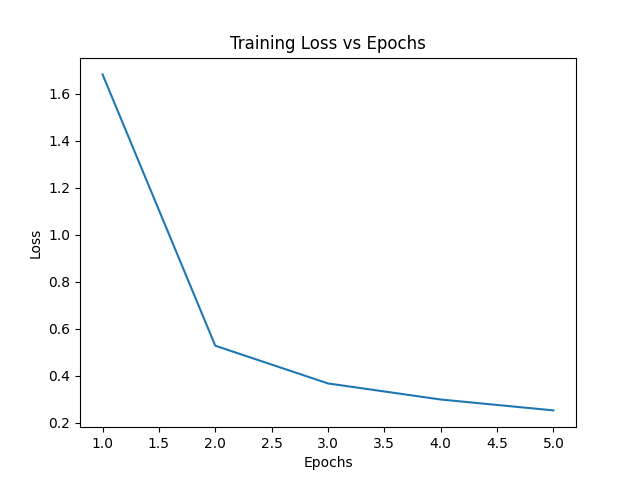
\includegraphics[width=0.9\columnwidth]{loss_epochs.png}
    \caption{Average training loss per epoch on 1000 MNIST samples.}
    \label{fig:loss_curve}
\end{figure}

\begin{figure}[htbp]
    \centering
    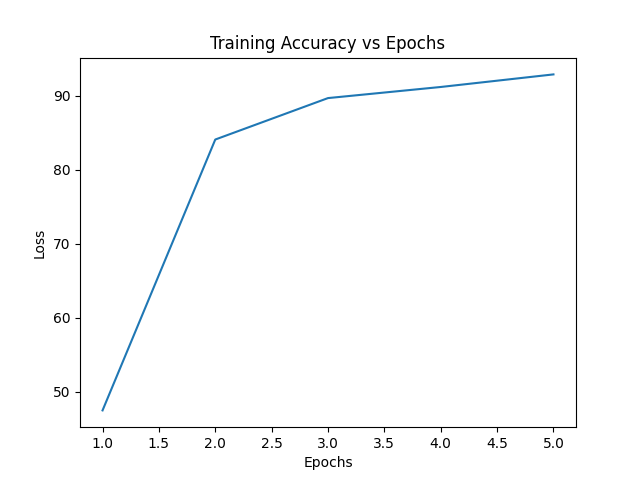
\includegraphics[width=0.9\columnwidth]{accuracy_epochs.png}
    \caption{Training accuracy per epoch on 1000 MNIST samples.}
    \label{fig:accuracy_curve}
\end{figure}

\subsubsection{Test Performance}
After 5 epochs of training, the model was evaluated on the 1000 unseen test samples.
\begin{itemize}
    \item \textbf{Test Accuracy}: 83.7\% (837 out of 1000 samples correctly classified).
    \item \textbf{Average Test Loss}: 0.52.
\end{itemize}
A confusion matrix for the test set predictions is presented in Fig. \ref{fig:confusion_matrix} to provide insight into which digits were commonly misclassified.

\begin{figure}[htbp]
    \centering
    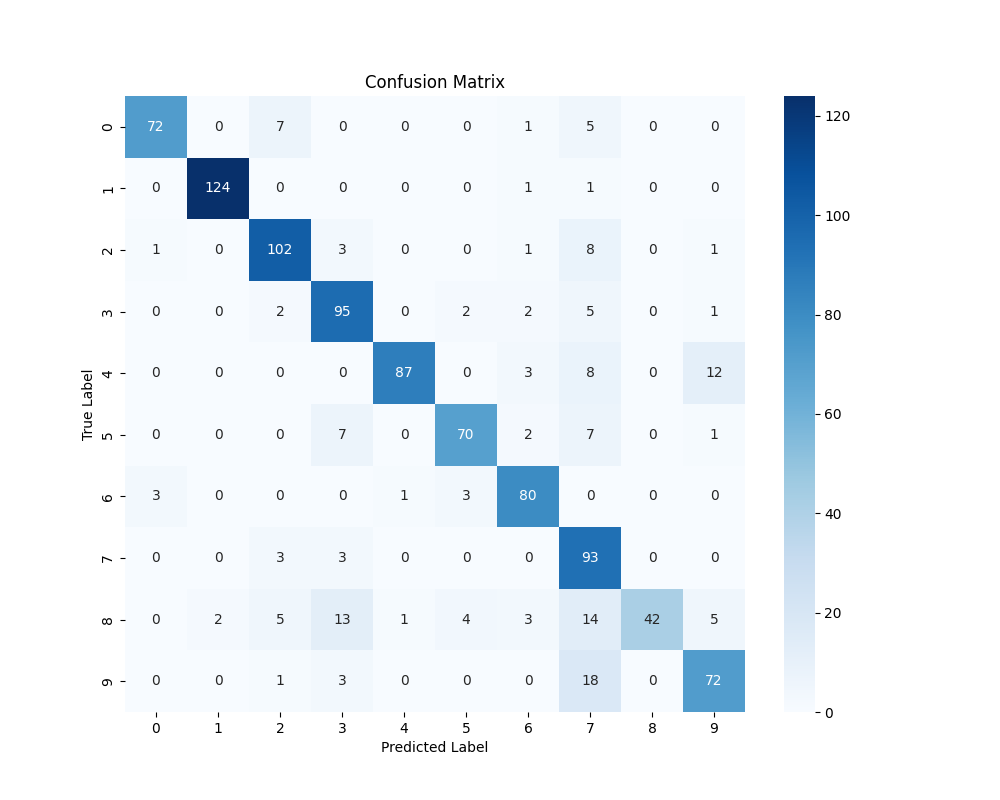
\includegraphics[width=0.9\columnwidth]{confusion_matrix.png}
    \caption{Confusion matrix for predictions on 1000 MNIST test samples.}
    \label{fig:confusion_matrix}
\end{figure}

\subsubsection{Execution Time}
The training process for 1,000 samples over 5 epochs took approximately 4 minutes to complete. 

The results demonstrate that even a simple CNN implemented from scratch can learn to classify MNIST digits with reasonable accuracy on a small subset of data. The training loss decreased and accuracy increased consistently over epochs, indicating successful learning. The test accuracy, while not state-of-the-art (which is expected given the simple architecture, small dataset, and from-scratch nature), is significantly above random chance (10\%) and validates the correctness of the core implementation. The prolonged training time is a key finding, highlighting the performance benefits of optimized numerical libraries.

\section{Discussion}
\subsection{Analysis of Results}
The training process, as evidenced by the decreasing loss (Fig. \ref{fig:loss_curve}) and increasing accuracy (Fig. \ref{fig:accuracy_curve}) over 5 epochs (Table \ref{tab:training_progress}), clearly indicates that the network was able to learn distinguishing features from the MNIST training samples. An initial training accuracy of 47.5\% after the first epoch improved to 92.9\% by the fifth epoch. This learning trend validates the correctness of the implemented forward and backward propagation mechanisms across the convolutional, ReLU, max-pooling, flatten, and dense layers.

The test accuracy of 83.7\% on a previously unseen subset of 1000 test images, while modest compared to state-of-the-art models built with optimized libraries, is significantly above the 10\% accuracy of random guessing. This performance further confirms that the network generalized to some extent from the training data. The drop from training accuracy to test accuracy (92.9\% vs. 83.7\%) is expected and indicates a degree of overfitting, which is common, especially with limited training data and a simple model without regularization techniques. The confusion matrix (Fig. \ref{fig:confusion_matrix}) would further reveal specific digit pairs that the model found harder to distinguish (e.g., 7 vs. 9, or 3 vs. 8).

\subsection{Challenges and Limitations}
Implementing a CNN from scratch presented several challenges and has inherent limitations:

\begin{itemize}
    \item \textbf{Computational Inefficiency}: The most significant challenge and limitation is the extreme computational cost. Performing tensor operations (convolutions, matrix multiplications) using nested Python loops is orders of magnitude slower than using optimized C/Fortran backends provided by libraries like NumPy, or GPU-accelerated operations in TensorFlow/PyTorch. The reported training time of approximately 4 minutes for 1,000 samples over 5 epochs highlights this inefficiency. Scaling this approach to larger datasets or more complex architectures would be practically infeasible.
    \item \textbf{Implementation Complexity and Debugging}: Manually implementing backpropagation for each layer, especially the convolutional layer, is intricate and prone to errors. Ensuring correct gradient calculations, tensor dimension handling, and indexing requires meticulous attention to detail. Debugging involved extensive manual checks of intermediate values and gradient flows.
    \item \textbf{Numerical Stability}: While not a major issue with this simple architecture and dataset, from-scratch implementations can be more susceptible to numerical stability problems (e.g., vanishing/exploding gradients, issues with softmax stability) without careful implementation of numerical tricks commonly found in established libraries.
\end{itemize}

\subsection{Insights Gained}
Despite the challenges, the from-scratch implementation yielded valuable insights:

\begin{itemize}
    \item \textbf{Deepened Understanding of Core Mechanics}: The process provided a profound understanding of how each layer transforms data during the forward pass and how gradients are computed and propagated during the backward pass. The role of the chain rule in backpropagation became explicitly clear.
    \item \textbf{Appreciation for Optimized Libraries}: The stark contrast in performance with library-based implementations underscores the immense value of optimized numerical computation libraries and GPU acceleration in practical deep learning.
    \item \textbf{Demystification of CNN Components}: The "black box" nature of library functions was peeled away, revealing the underlying algorithms for convolution, pooling, activation, and dense connections.
    \item \textbf{Intuition for Hyperparameter Effects}: Manually coding the update rules provided a more direct sense of how hyperparameters like the learning rate affect the training process.
\end{itemize}
This exercise effectively served its primary educational purpose of solidifying foundational knowledge in neural network operations.

\section{Conclusion and Future Work}
This project successfully detailed the design, implementation, and evaluation of a simple Convolutional Neural Network from scratch for classifying MNIST handwritten digits. Using only fundamental Python constructs, we demonstrated the functional implementation of core CNN components, including convolutional, ReLU activation, max-pooling, flatten, and dense layers, along with the backpropagation algorithm for training. The network achieved a test accuracy of 83.7\% on a subset of the MNIST test data after 5 epochs of training, confirming its ability to learn and generalize.

The primary contribution lies in the educational value of this from-scratch approach, which provided a deep and practical understanding of the internal workings of CNNs. While the computational performance was significantly slower than library-based solutions, this limitation itself served to highlight the critical role of optimized numerical libraries in modern deep learning. The project successfully demystified the core operations within a CNN, offering valuable insights into data transformation and gradient flow.

\end{document}
